\chapter{Experiments and Evaluation} \label{sec:ch_eval}

Experiments that were performed to evaluate our methods and approaches will be presented in this chapter. Four main sections separate the experiments by topic, to which they belong.

\section{Evaluation of Manual Rules} \graphicspath{{../img/ch50/}}


In this section, several experiments will be presented to explain the usefulness of our extraction method based on manually designed rules. 



Two experiments with manually created extraction rules will be presented in this section. The first one provides measurements on a higher amount of texts without manual gold standard annotations, while the second experiment was done on a small manually annotated collection. 

\subsection{Czech Fireman Quantitative} \label{sec:ch50_quant_experiment}

We evaluated three extraction rules (one procedural and two Netgraph based) on a set of 814 texts of news of several Czech fire departments and measured several statics. All the rules had the same goal: to find numbers of people that died or were injured during an accident. The procedural rule was the same as in Figure~\ref{lst:btred_rule} and the Netgraph based rules correspond with the rule in Figure~\ref{fig:ch50_extract_patern}. The only difference between the Netgraph rules is that in the first case (Netgraph 1) all rule nodes except number 1 (\verb+action_type+) were set as optional, while in the second case (Netgraph 2) also node 4 (participant) was compulsory. This little change caused some interesting effects -- see below. 

Table~\ref{tab:ch50_tab_manual_rules} summarizes some of the statics that were measured. Description of individual values follows.

\begin{table}
	\centering
		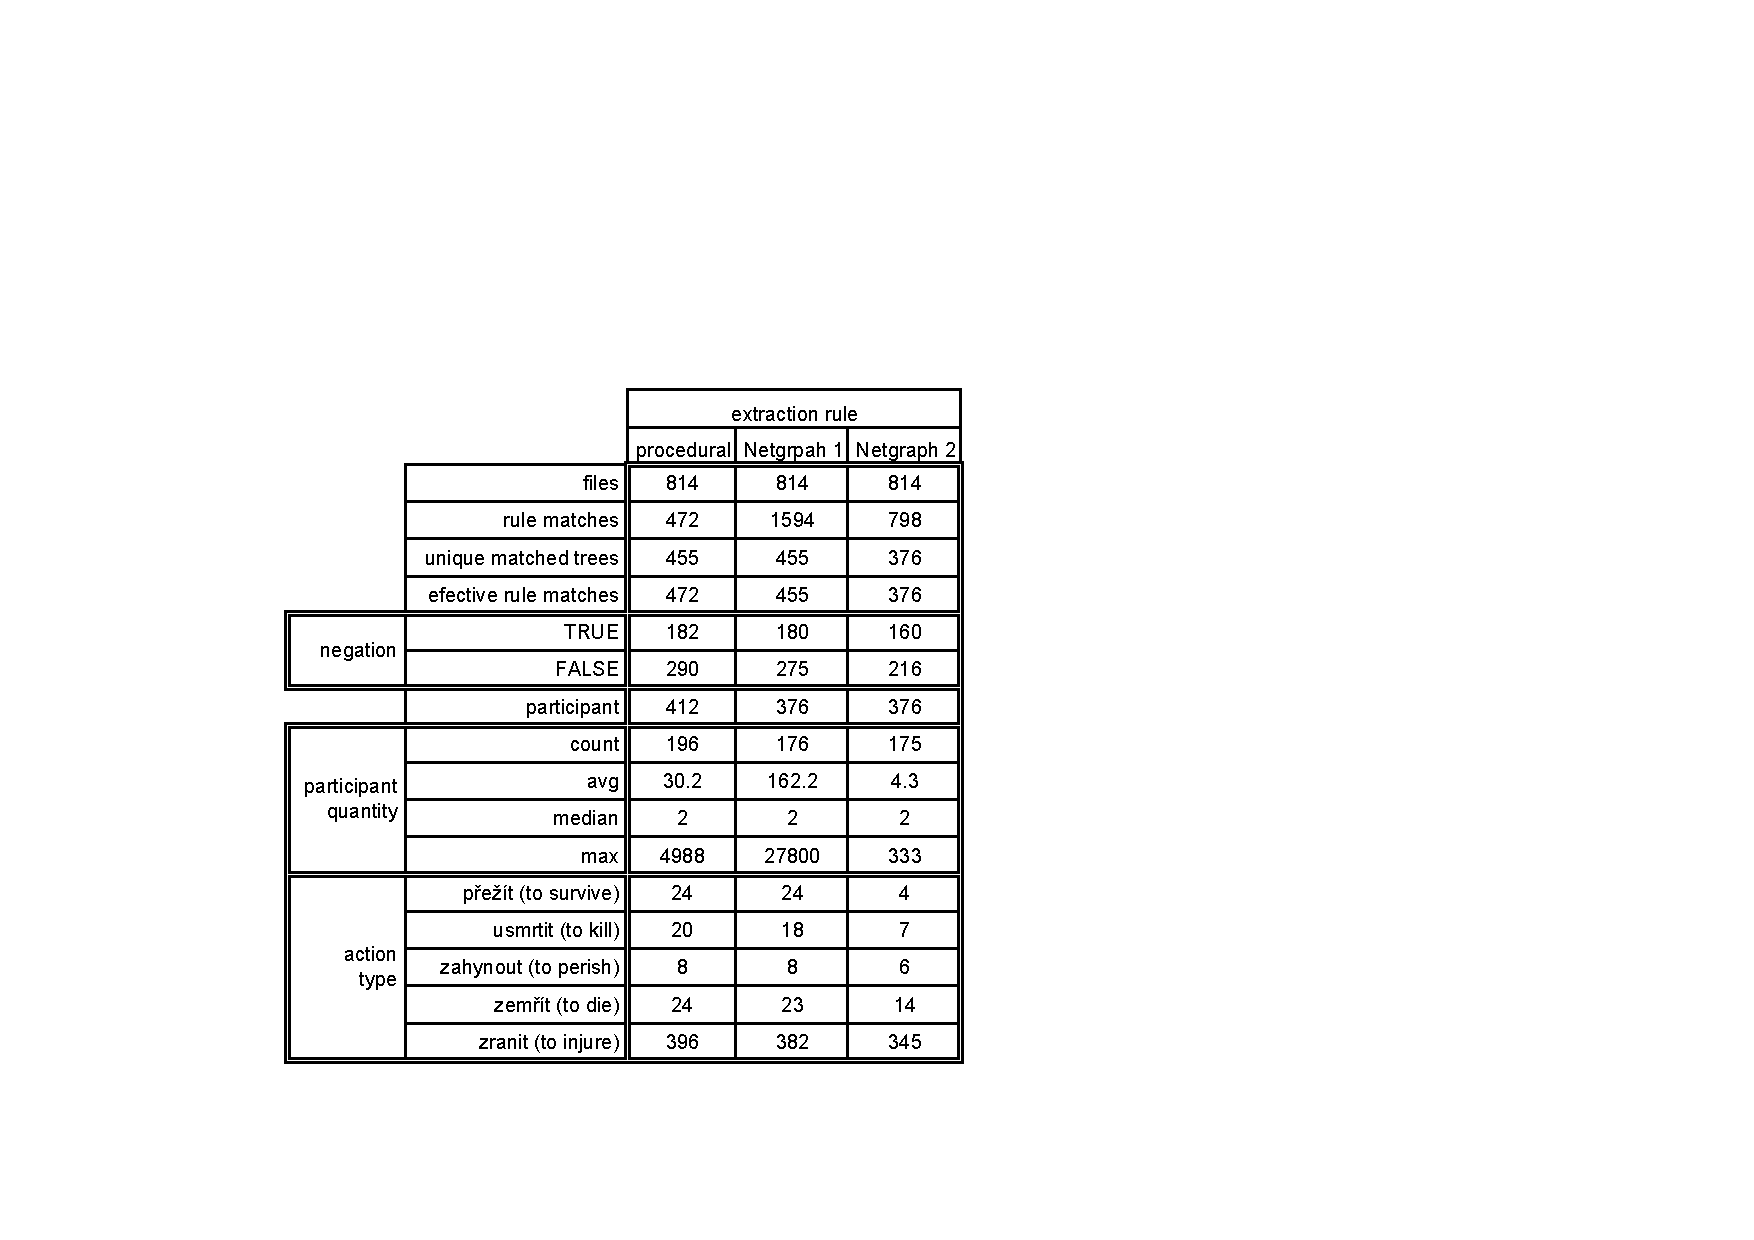
\includegraphics[angle=-90,width=0.6\hsize]{tab_manual_rules}
	\caption{Evaluation of manually created rules (bigger dataset without manual annotations).}
	\label{tab:ch50_tab_manual_rules}
\end{table}


\begin{description}
	\item[Files]
The same set of 814 files (texts) was used in all the experiments.

	\item[Rule matches]
The presence of optional nodes in a query increases the number of possibilities how a Netgraph query can be matched to a single linguistic tree. An optional node might or might not be marked in the result. The number of possible matches is also increased if there are more compatible nodes in a candidate tree that can be matched with a single query node. This can even be true for the participant query node (4) in the case of Netgraph based rules if a sentence mentions more than one affected person. This can be marked as a mistake in the rule design -- it does not count with such possibility, or it can be taken as a drawback of the current evaluation algorithm of the Netgraph based method -- it should put all the possibilities to the output. Note that this issue does not concern the procedural method, which outputs all the matching participants.

	\item[Unique matched trees]
This number represents the number of unique trees matched by the extraction rule.

	\item[Effective rule matches]
Because the procedural rules and the Netgraph based rules are evaluated in a different way, the way of selection of effective matches (matches that are used for the output) is also different. In the procedural case all matches are used because every such match is tied up with a different verb in a sentence. In this case more matches per sentence (tree) are only possible for complex sentences with more verbs and therefore every match is applicable because it is connected with a different piece of information.\\
In the Netgraph case it is necessary to select the most relevant matches of all possible ones. The first longest (maximum of optional nodes) match for each tree is selected. This is unfortunately not optimal and also not consistent with the procedural case, but it is the easiest option for the implementation (Netgraph can be directly used in that case.)

	\item[Negation, participant, participant quantity (count), action type]
These values represent numbers of matching nodes (or more precisely of pieces of extracted information) of the given type. For example values of participant are the numbers of all participants (node number 4 in the Netgraph based rule) identified by the extraction rule and values of \emph{p�e��t} (survive) are numbers of matching action type nodes with the value of \emph{p�e��t} (survive). Note that some postprocessing of the Netgraph based output was necessary to count TRUE and FLASE negation values.

	\item[Participant quantity]
Values in this group are all connected with the quantity kind of information. It expresses the quantity of participants involved in the corresponding incident action. This kind of information is numeric so some numerical calculations can be made (average value, median and maximum value). Again postprocessing of the Netgraph based output was necessary to obtain these values -- in this case translation of seven kinds of numerals to numbers (\emph{jeden} - 1, \emph{dva} - 2, \emph{t�i} - 3, \emph{�ty�i} - 4, \emph{�est} - 6, \emph{sedm} - 7, \emph{osm} - 8). Note that the vale of average is strongly affected by the very few high numbers present in the results (the values 1 and 2 accounted for more than half of the results.)\\
Values of participant quantity also demonstrate several errors made by the particular extraction rules, see bellow for details.
\end{description}





















\subsubsection{Detected errors}

Results of the extraction were investigated only partly; no formal evaluation is available in this case (except on a small evaluation set, see bellow: the second experiment). About 10-20\% of information was not extracted because of errors of linguistic parsing; majority of the errors was made in long complex sentences, which are known to be difficult for linguistic processing. There was only a few of false positives. A nice example can be traced from the maximum values of participant quantity in Table 99. Three different numbers were found in the three experiments: 27800, 4988 and 333. The number of 27800 is actually a number of chickens that died during one of the accidents. The number was extracted by the first Netgraph based rule because the query node 4 (participant) was marked as optional and omitted during the evaluation. This node normally ensures that the participant is one of: person, man, woman, child, driver, etc.
Numbers 4988 and 333 are both correct. They were both used in the same sentence, which summarized numbers of injured (4988) and killed (333) people during one whole year. Although the sentence was quite complex it was linguistically parsed correctly and also the procedural rule managed to extract both numbers correctly. The Netgraph based rule extracted only the first number in the sentence because the current evaluation algorithm does not allow multiple matches per sentence (see above the comments of rule matches and effective rule matches).


\subsection{Czech Fireman Qualitative}


\begin{table}
	\centering
	\begin{tabular}{|r|c|c|c|c|c|c|}
		\hline
		 & correct & missing & spurious & recall & precision & $F_1$\\
		\hline
		injuries & 3 & 29 & 0 & 0.09 & 1 & 0.17\\
		\hline
		fatalities & 1 & 10 & 0 & 0.09 & 1 & 0.17\\
		\hline
	\end{tabular}
	\caption{Evaluation of the manually created rule form Figure~\ref{fig:ch50_extract_patern} on the manually annotated dataset.}
	\label{tab:ch50_extract_patern_eval}
\end{table}



In the second experiment a manually annotated collection of 50 fireman news texts was used. Having the extraction rule from the previous experiment and a set of manually annotated texts it is only natural to ask a question about the success of the extraction rule on that collection. Table~\ref{tab:ch50_extract_patern_eval} summarizes the results. These results are far from satisfactory; the recall of 0.09 is something that is far from any acceptable use. Several explanations of the issue can be provided. The extraction rule serves more for a demonstration than for exhausting coverage of all possible cases. The extraction rule looks for particular verb (to injure, to die, etc.) but the information can be also expressed by an adjective (injured driver, death passenger, etc.); another extraction rules should be constructed for these and other cases. The training collection used for the design was also of a different spectrum of texts.



On the other hand this experiment shows how a manually annotated collection contributes to the quality of extraction rules. We can never know if the extraction rule is usable until a formal evaluated is made. Also the fact that the precision is strictly 1 should be noted. This means that the extraction rule made no mistake in those cases when it provided some output.



\subsubsection{Manual Design of Rules Using Training Data Set}  

\begin{table}
	\centering
	\begin{tabular}{|r|c|c|c|c|c|c|}
		\hline
		 & correct & missing & spurious & recall & precision & $F_1$\\
		\hline
		manual rules & 5 & 2 & 0 & 0.71 & 1 & 0.83\\
		\hline
		ILP rules & 5 & 2 & 0 & 0.71 & 1 & 0.83\\
		\hline
	\end{tabular}
	\caption{Evaluation of the manually created rules and ILP learned rules (manually annotated dataset was used for rule design (training half) and evaluation (testing half) -- see the description of the second experiment in text.)}
	\label{tab:ch50_damage_manual_eval}
\end{table}

\begin{table}
	\centering
	\begin{tabular}{|r|c|c|c|c|c|c|}
		\hline
		 & correct & missing & spurious & recall & precision & $F_1$\\
		\hline
		manual rules & 4 & 1 & 1 & 0.8 & 0.8 & 0.8\\
		\hline
		ILP rules & 4 & 1 & 1 & 0.8 & 0.8 & 0.8\\
		\hline
	\end{tabular}
	\caption{Cross method comparison of found instances.}
	\label{tab:ch50_damage_cross_method}
\end{table}




Next question that naturally emerges is: How would be the performance if the rules were designed with the support of a manually annotated collection? An additional experiment was made to answer that question. The collection was split into two even parts -- training part and testing part. A manually created rule was designed so that it correctly matched with all annotations of the training part and then it was evaluated on the testing part. For the validity of the experiment it was necessary that the designer did not have any knowledge about the data of the testing part; that is why we used a different extraction task (damage instead of injuries and fatalities).We have also compared the performance of the manually created rule with a rule learned by the ILP machine learning engine (see Chapter~\ref{ch:ILP_Learning}).

The results are summarized in Table~\ref{tab:ch50_damage_manual_eval}. Both kinds of rules (manually designed and learned by ILP) performed the same (recall: 0.71, precision: 1); both the methods correctly found 5 instances and they were both unable to find 2 instances. From the cross coverage comparison in 
Table~\ref{tab:ch50_damage_cross_method} it is apparent that the methods agreed on 4 instances and each method was able to discovered one instance that the other did not discover. Such results could be accepted for a practical application but we must not forget the fact that the collection is very small and only single evidence is provided by the experiment, so it dies not provide any statistical significance (getting statistically significant results would require experiments with different datasets, extraction tasks and human designers.) 



\section{Evaluation of Learned Rules}

\subsection{Czech Fireman Performance}

\subsection{Acquisitions Performance}

\subsection{?Acquisitions Time?}











\clearpage

%%%%%%%%%%%%%%%%%%%%%%%%%%%%%%%%%%%%%%%%%%%%%%%%%%%%%%%%%%%%%%%%%%%%%%%%%%%%%%%%%%%%%%%%%%%%%%%%%%%%%%%%%%%%%%
%%%%%%%%%%%%%%%%%%%%%%%%%%%%%%%%%%%%%%%%%%%%%%%%%%%%%%%%%%%%%%%%%%%%%%%%%%%%%%%%%%%%%%%%%%%%%%%%%%%%%%%%%%%%%%
%%%%%%%%%%%%%%%%%%%%%%%%%%%%%%%%%%%%%%%%%%%%%%%%%%%%%%%%%%%%%%%%%%%%%%%%%%%%%%%%%%%%%%%%%%%%%%%%%%%%%%%%%%%%%%
\section{Evaluation of Shareable Extraction Ontologies Performance} \label{sec:eval_Shareable_Extraction_Ontologies} \label{sec:ch70_experiment}

In this section we present an experiment that should serve as a proof of a concept that the proposed idea of independent extraction ontologies is realizable. We have selected several reasoners (namely Jena, HermiT, Pellet and FaCT++) and tested them on two slightly different datasets from two different domains and languages (see Table~\ref{tab:datasets}). This should at least partially demonstrate the universality of the proposed approach.

In both cases the task is to find all instances (corresponding to words in a document) that should be uncovered by the extraction rules. The extraction rules are saved in single extraction ontology for each dataset. The datasets are divided into individual document ontologies (owl files) corresponding to the individual documents. During the experiment the individual document ontologies are processed separately (one ontology in a step) by a selected reasoner. The total time taken to process all document ontologies of a dataset is the measured result of the reasoner for the dataset.

The actual reasoning tasks are more difficult than a simple retrieval of all facts entailed by the extraction rules. Such simple retrieval task took only a few seconds for the Acquisitions v1.1 dataset (including parsing) in the native Prolog environment that the IE engine uses. There were several more inferences needed in the reasoning tasks because the schema of the input files was a little bit different from the schema used in rules. The mapping of the schemas was captured in another ``mapping'' ontology that was included in the reasoning. The mapping ontology is a part of the publically available project ontologies.
%\footnote{See ``Data/ontologies'' link on the project page \url{http://czsem.berlios.de/}}%and a potentially interested reader can find the complete mapping ontology on the project's web site.


\subsection{Datasets} \label{sec:ch70_datasets}

In the experiment we used two slightly different datasets from two different domains and languages.  Table~\ref{tab:datasets} summarizes some basic information about them. The fist dataset is called `czech\_fireman', it is based on Czech texts that are reporting on fire and traffic accidents and it was already described in Section~\ref{sec:ch40_rdf_fireman}. The second dataset is called ``Corporate Acquisition Events'', it is based on news articles describing acquisition events, taken from the Reuters dataset and it was already described in Section~\ref{sec:ch40_rdf_acquisitions}.

\begin{table}
\begin{center}
\begin{tabular}{|r||l|l|b{20mm}|b{20mm}|b{20mm}|}
%\begin{tabular}{|r||r|r|c|r|c|}
\hline
dataset & domain & language & number of~files &  dataset size (MB) &  number of~rules  \\
\hline
\hline
\textbf{czech\_fireman} & accidents & Czech &  50 &  16 &  2\\
\hline
\textbf{acquisitions} & finance & English &  600 &  126 &  113\\
\hline
\end{tabular}
\caption{Description of datasets that were used.}\label{tab:datasets}
\end{center}
\end{table}




\subsection{Reasoners}

%In the experiment we used four OWL reasoners
Four OWL reasoners were used in the experiment(namely
Jena\footnote{\url{http://jena.sourceforge.net}}
,HermiT\footnote{\url{http://hermit-reasoner.com}}
,Pellet\footnote{\url{http://clarkparsia.com/pellet}}
and FaCT++\footnote{\url{http://code.google.com/p/factplusplus}}
) and the time they spent on processing a particular dataset was measured. The time also includes time spent on parsing the input. HermiT, Pellet and FaCT++ were called through OWL API-3.1, so the same parser was used for them. Jena reasoner was used in its native environment with the Jena parser.
In the early beginning of the experiment we had to exclude the FaCT++ reasoner from both tests. It turned out that FaCT++ does not work with rules\footnote{\url{http://en.wikipedia.org/wiki/Semantic_reasoner#Reasoner_comparison}} and it did not return any result instances.  All the remaining reasoners strictly agreed on the results and returned the same sets of instances.

Also HermiT was not fully evaluated on the Acquisitions v1.1 dataset because it was too slow. The reasoner spent 13 hours of running to process only 30 of 600 files of the dataset. And it did not seem useful to let it continue. We contacted the authors of HermiT to clarify this issue and we were reminded that HermiT was mainly designed as a TBox reasoner and it was particularly optimized for the ontology classification problem \citep{ghms10classification}; it was never optimized for simple rule based (ABox) inferences.












\subsection{Evaluation Results}



\begin{table}
\begin{center}
\begin{tabular}{|r||r|r||r|r|}
\hline
reasoner & \textbf{czech\_fireman} & stdev & \textbf{acquisitions-v1.1} & stdev\\
\hline
\hline
\textbf{Jena} & 161 s & 0.226 & 1259 s & 3.579\\
\hline
\textbf{HermiT} & 219 s & 1.636 & $\gg$ 13 hours & \\
\hline
\textbf{Pellet} & 11 s & 0.062 & 503 s & 4.145\\
\hline
\textbf{FaCT++} & \multicolumn{4}{|c|}{Does not support rules.}\\
\hline
\end{tabular}
\end{center}

Time is measured in seconds. Average values from 6 measurements. Experiment environment: Intel Core I7-920 CPU 2.67GHz, 3GB of RAM, Java SE 1.6.0\_03, Windows XP.

\caption{Time performance of tested reasoners on both datasets.}
\label{tab:results}
\end{table}

Table~\ref{tab:results} summarizes results of the experiment. The standard deviations are relatively small when compared to the differences between the average times.  So there is no doubt about the order of the tested reasoners. Pellet performed the best and HermiT was the slowest amongst the tested and usable reasoners in this experiment.

From the results we can conclude that similar tasks can be satisfactorily solved by contemporary OWL reasoners because three of four tested reasoners were working correctly and two reasoners finished in bearable time.

On the other hand even the fastest system took 8.5 minutes to process 113 rules over 126MB of data. This is clearly   significantly longer than a operational system would require. 
Contemporary Semantic Web reasoners are known still to be often quite inefficient and the experiment showed that using them today to do information extraction will result in quite poor performance. However, efficiency problems can be solved
and in the context of Linked Data providing shareable descriptions of information extraction rules may be valuable.















%%%%%%%%%%%%%%%%%%%%%%%%%%%%%%%%%%%%%%%%%%%%%%%%%%%%%%%%%%%%%%%%%%%%%%%%%%%%%%%%%%%%%%%%%%%%%%%%%%%%%%%%%%%%%%
%%%%%%%%%%%%%%%%%%%%%%%%%%%%%%%%%%%%%%%%%%%%%%%%%%%%%%%%%%%%%%%%%%%%%%%%%%%%%%%%%%%%%%%%%%%%%%%%%%%%%%%%%%%%%%
%%%%%%%%%%%%%%%%%%%%%%%%%%%%%%%%%%%%%%%%%%%%%%%%%%%%%%%%%%%%%%%%%%%%%%%%%%%%%%%%%%%%%%%%%%%%%%%%%%%%%%%%%%%%%%
\section{Evaluation of Fuzzy ILP Classification} \label{sec:ch80_eval}
\graphicspath{{../img/ch80/}}

\begin{figure}[p]
\centerline{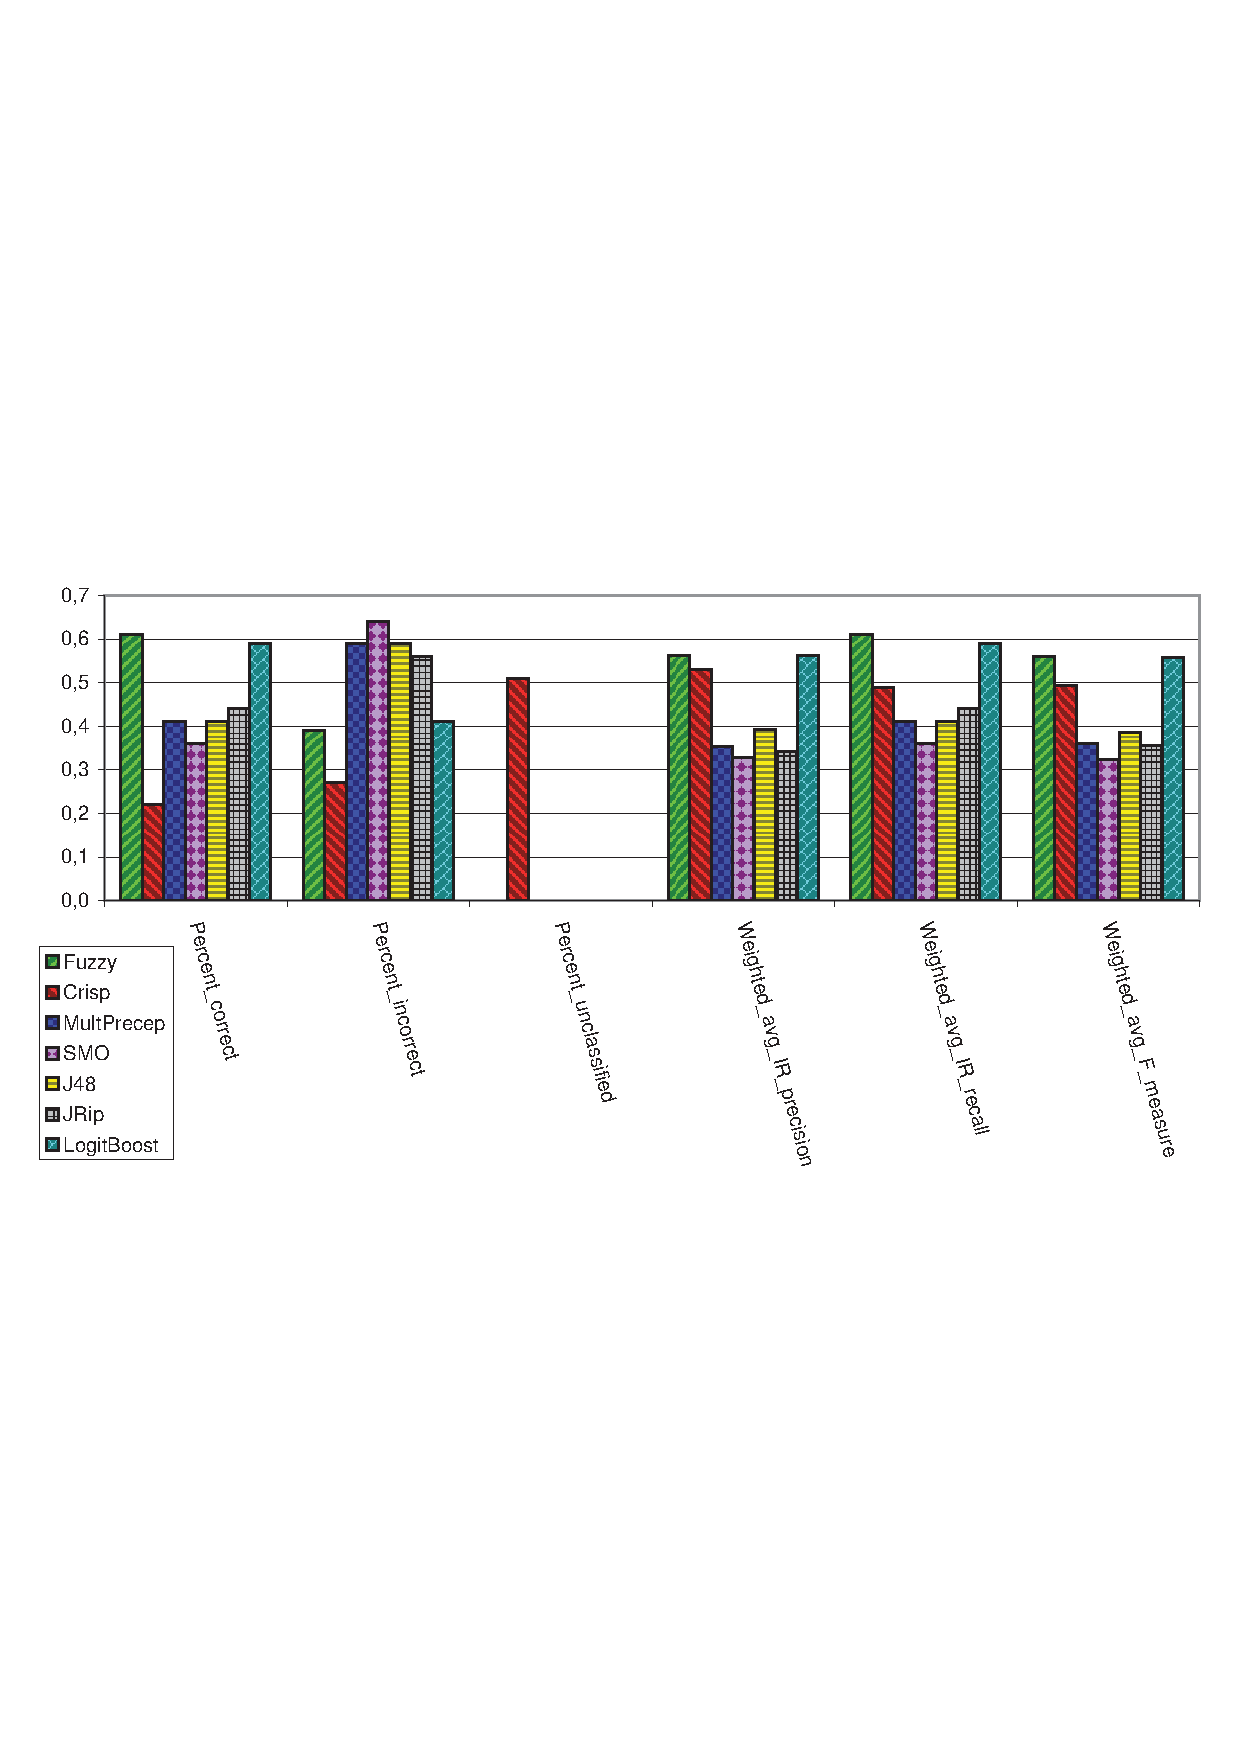
\includegraphics[width=0.8\hsize]{2x10cross}}
\caption{Evaluation of the methods -- average values.}
\label{img:graph2x10}
\end{figure}


\begin{table}[p]
\scriptsize
{\centering \begin{tabular}{lr@{\hspace{0cm}}c@{\hspace{0cm}}rr@{\hspace{0cm}}c@{\hspace{0cm}}r@{\hspace{0.05cm}}cr@{\hspace{0cm}}c@{\hspace{0cm}}r@{\hspace{0.05cm}}cr@{\hspace{0cm}}c@{\hspace{0cm}}r@{\hspace{0.05cm}}cr@{\hspace{0cm}}c@{\hspace{0cm}}r@{\hspace{0.05cm}}cr@{\hspace{0cm}}c@{\hspace{0cm}}r@{\hspace{0.05cm}}cr@{\hspace{0cm}}c@{\hspace{0cm}}r@{\hspace{0.05cm}}c}
\hline
& \multicolumn{3}{c}{Fuzzy}& \multicolumn{4}{c}{Crisp} & \multicolumn{4}{c}{MultPerc} & \multicolumn{4}{c}{SMO} & \multicolumn{4}{c}{J48} & \multicolumn{4}{c}{JRip} & \multicolumn{4}{c}{LBoost} \\
\hline
Corr	& 0.61 & $\pm$ & .19 & .22 & $\pm$ & .17 & $\bullet$ & .41 & $\pm$ & .19 & $\bullet$ & .36 & $\pm$ & .24 & $\bullet$ & .41 & $\pm$ & .22 & $\bullet$ & .44 & $\pm$ & .17 & $\bullet$ & .59 & $\pm$ & .26 &        \\
Incor	&  .39 & $\pm$ & .19 & .27 & $\pm$ & .24 &         	 & .59 & $\pm$ & .19 & $\circ$ 	 & .64 & $\pm$ & .24 & $\circ$ 	 & .59 & $\pm$ & .22 & $\circ$ 	 & .56 & $\pm$ & .17 & $\circ$ 	 & .41 & $\pm$ & .26 &        \\
Uncl	&  .00 & $\pm$ & .00 & .51 & $\pm$ & .29 & $\circ$   & .00 & $\pm$ & .00 &         	 & .00 & $\pm$ & .00 &         	 & .00 & $\pm$ & .00 &         	 & .00 & $\pm$ & .00 &         	 & .00 & $\pm$ & .00 &        \\
Prec	&  .56 & $\pm$ & .24 & .53 & $\pm$ & .37 &         	 & .35 & $\pm$ & .20 & $\bullet$ & .33 & $\pm$ & .26 &         	 & .39 & $\pm$ & .22 &         	 & .34 & $\pm$ & .21 & $\bullet$ & .56 & $\pm$ & .28 &        \\
Rec		&  .61 & $\pm$ & .19 & .49 & $\pm$ & .32 &         	 & .41 & $\pm$ & .19 & $\bullet$ & .36 & $\pm$ & .24 & $\bullet$ & .41 & $\pm$ & .22 & $\bullet$ & .44 & $\pm$ & .17 & $\bullet$ & .59 & $\pm$ & .26 &        \\
F			&  .56 & $\pm$ & .20 & .49 & $\pm$ & .33 &         	 & .36 & $\pm$ & .19 & $\bullet$ & .32 & $\pm$ & .24 & $\bullet$ & .39 & $\pm$ & .21 &         	 & .36 & $\pm$ & .19 & $\bullet$ & .56 & $\pm$ & .27 &        \\
\hline
\multicolumn{21}{c}{$\circ$, $\bullet$ statistically significant increase or decrease}\\
\end{tabular} \scriptsize \par}
\scriptsize
\smallskip
Legend:\\
{\centering
\begin{tabular}{p{2cm}@{}p{10.5cm}}\\
Fuzzy \dotfill{}& czsem.ILP.FuzzyILPClassifier '' \\
Crisp \dotfill{} & czsem.ILP.CrispILPClassifier '' \\
MultPerc \dotfill{} & functions.MultilayerPerceptron '-L 0.3 -M 0.2 -N 500 -V 0 -S 0 -E 20 -H a' \\
SMO \dotfill{} & functions.SMO '-C 1.0 -L 0.0010 -P 1.0E-12 -N 0 -V -1 -W 1 -K \textbackslash"functions.supportVector.PolyKernel -C 250007 -E 1.0\textbackslash"' \\
J48 \dotfill{} & trees.J48 '-C 0.25 -M 2' \\
JRip \dotfill{} & rules.JRip '-F 3 -N 2.0 -O 2 -S 1' \\
LBoost \dotfill{} & meta.LogitBoost '-P 100 -F 0 -R 1 -L -1.7976931348623157E308 -H 0.1 -S 1 -I 10 -W trees.DecisionStump' \\
\\
Corr \dotfill{} & Percent correct\\
Inor \dotfill{} & Percent incorrect\\
Uncl \dotfill{} & Percent unclassified\\
Prec \dotfill{} & IR precision, weighted average from all classes\\
Rec \dotfill{} 	& IR recall, weighted average from all classes\\
F \dotfill{} 		& F measure, weighted average from all classes\\
\end{tabular}
}
\caption{Evaluation of the methods in 2 times 10-fold cross validation.}
\label{tab:table2x10}
\end{table}


We have evaluated both ILP methods and compared them with other machine learning procedures used in data mining. To make the comparison clear and easy to perform, we have implemented an interface between the ILP methods and Weka (Section~\ref{sec:ch30_weka}). This interface makes it possible to use the ILP methods as an ordinary Weka classifier for any\footnote{For the fuzzy ILP method, there is a requirement on the target (class) attribute: it has to be monotonizable (e.g. numeric).} classification task inside the Weka software. This also makes the presented experiments easily repeatable (see Secrion~\ref{sec:ch90_repeatablity} for details.) 



\subsection{Czech Fireman Performance}


For our experiment we used the Weka Experimenter (see in Section~\ref{sec:ch30_weka}) and performed an experiment in which the Crisp and Fuzzy ILP classifiers were compared with five additional classifiers:
\begin{itemize}
	\item Multilayer Perceptron \citep{biblio:bishop-1995},
	\item Support Vector Machine classifier SMO \citep{biblio:SMO},
	\item J48 decision tree \citep{biblio:J48},
	\item JRip rules \citep{weka:JRip} and
	\item Additive logistic regression LogitBoost \citep{biblio:LogitBoost}.
\end{itemize}
We have evaluated all the methods two times by 10-fold cross validation. %(section~\ref{sec:experiment_desc}).
The obtained results (average values) are described by the graph in Figure~\ref{img:graph2x10} and in Table~\ref{tab:table2x10} (with standard deviations and marked statistically significant values).

There is no clear winner in our experiment. But the Fuzzy ILP classifier proved better results than a majority of the methods on our data and the results are statistically significant in many cases. Very good results were also obtained using LogitBoost. 





\begin{table}
\scriptsize
{\centering \begin{tabular}{l|r@{\hspace{0cm}}c@{\hspace{0cm}}r@{\hspace{0.3cm}}r@{\hspace{0cm}}c@{\hspace{0cm}}r@{\hspace{0.05cm}}cr@{\hspace{0cm}}c@{\hspace{0cm}}r@{\hspace{0.05cm}}l@{\hspace{0cm}}r@{\hspace{0cm}}c@{\hspace{0cm}}r@{\hspace{0.05cm}}cr@{\hspace{0cm}}c@{\hspace{0cm}}r@{\hspace{0.05cm}}cr@{\hspace{0cm}}c@{\hspace{0cm}}r@{\hspace{0.05cm}}cr@{\hspace{0cm}}c@{\hspace{0cm}}r@{\hspace{0cm}}c@{\hspace{0.25cm}}c@{\hspace{0.20cm}}c@{\hspace{0.10cm}}}
& \multicolumn{3}{c}{Fuzzy}& \multicolumn{4}{c}{Crisp} & \multicolumn{4}{c}{MultPerc} & \multicolumn{4}{c}{SMO} & \multicolumn{4}{c}{J48} & \multicolumn{4}{c}{JRip} & \multicolumn{4}{c}{LBoost} & train & test\\
\hline
car & .39 & $\pm$ & .03 & .36 & $\pm$ & .03 & $\bullet$ & .53 & $\pm$ & .02 & $\circ$ & .57 & $\pm$ & .01 & $\circ$ & .50 & $\pm$ & .02 & $\circ$ & .51 & $\pm$ & .03 & $\circ$ & .54 & $\pm$ & .02 & $\circ$ & 173 & 1554\\
\hline
wine & .44 & $\pm$ & .03 & .42 & $\pm$ & .02 & $\bullet$ & .48 & $\pm$ & .02 & $\circ$ & .46 & $\pm$ & .02 & $\circ$ & .47 & $\pm$ & .02 & $\circ$ & .48 & $\pm$ & .03 & $\circ$ & .52 & $\pm$ & .02 & $\circ$ & 160 & 1439\\
\hline
cmc & .79 & $\pm$ & .02 & .77 & $\pm$ & .03 & $\bullet$ & .89 & $\pm$ & .02 & $\circ$ & .81 & $\pm$ & .01 & $\circ$ & .88 & $\pm$ & .02 & $\circ$ & .82 & $\pm$ & .03 & $\circ$ & .85 & $\pm$ & .02 & $\circ$ & 147 & 1325\\
\hline
tae & .50 & $\pm$ & .12 & .39 & $\pm$ & .11 & $\bullet$ & .59 & $\pm$ & .11 & $\circ$ & .55 & $\pm$ & .12 & $\circ$ & .50 & $\pm$ & .12 &  & .37 & $\pm$ & .11 & $\bullet$ & .55 & $\pm$ & .11 & $\circ$ & 135 & 15\\
\hline
pop & .66 & $\pm$ & .09 & .54 & $\pm$ & .17 & $\bullet$ & .57 & $\pm$ & .13 & $\bullet$ & .70 & $\pm$ & .06 & $\circ$ & .70 & $\pm$ & .07 & $\circ$ & .70 & $\pm$ & .06 & $\circ$ & .66 & $\pm$ & .10 &  & 80 & 9\\
\hline
nurs & .79 & $\pm$ & .04 & .68 & $\pm$ & .06 & $\bullet$ & .81 & $\pm$ & .04 & $\circ$ & .73 & $\pm$ & .04 & $\bullet$ & .80 & $\pm$ & .04 & $\circ$ & .79 & $\pm$ & .06 &  & .83 & $\pm$ & .02 & $\circ$ & 52 & 12907\\
\hline
\multicolumn{23}{c}{$\circ$, $\bullet$ statistically significant improvement or degradation}\\
\end{tabular} \scriptsize \par}
\scriptsize
\smallskip
Legend:\\
{\centering
\begin{tabular}{p{2cm}@{}p{10.5cm}}\\
train \dotfill{} & average number ($\pm$1) of training instances in each run\\
test \dotfill{} & average number ($\pm$1) of testing instances in each run\\
\\
car \dotfill{} & \url{http://archive.ics.uci.edu/ml/datasets/Car+Evaluation}\\
wine \dotfill{} & red wine dataset \url{http://archive.ics.uci.edu/ml/datasets/Wine+Quality}\\
cmc \dotfill{} & \url{http://archive.ics.uci.edu/ml/datasets/Contraceptive+Method+Choice}\\
tae \dotfill{} & \url{http://archive.ics.uci.edu/ml/datasets/Teaching+Assistant+Evaluation}\\
pop \dotfill{} & \url{http://archive.ics.uci.edu/ml/datasets/Post-Operative+Patient}\\
nurs \dotfill{} & \url{http://archive.ics.uci.edu/ml/datasets/Nursery}\\
\end{tabular}
}


\smallskip


Learning parameters for both ILP methods:\\set(noise,20). set(i,3). set(clauselength,13). set(search,heuristic). set(evalfn,wracc). set(samplesize,3).
\caption{Evaluation of the methods on UCI datasets, \textbf{percent correct}, average values from 100 repetitions.}
\label{tab:UCItable}
\end{table}


\subsection{UCI Performance}


The Fuzzy ILP classifier performed quite well on our dataset, but the next question is: How is it with other data, with more learning instances, and what about the time complexity? To answer these questions we performed another experiment. We selected several datasets from the UCI repository (see Section~\ref{sec:ch40_uci_datasets}) and evaluated all the methods against them. 



The list of selected datasets can be found in the legend of Table~\ref{tab:UCItable}. All the datasets are monotonizable (the target attribute can be naturally ordered), so the fuzzy classifier could take advantage of that. Learning settings are the same as before (Table~\ref{tab:table2x10}) except for settings of both ILP classifiers, which  performed a little bit better with modified settings on a majority of the datasets (see in the legend of Table~\ref{tab:UCItable}). 

Table~\ref{tab:UCItable} compares the numbers of correctly classified instances on all the datasets. The last two columns show numbers of training and testing instances. The numbers of training instances are quite low; this is because the ILP classifiers are probably not capable of fully exploiting higher numbers of training instances and the difference between ILP classifiers and the others would be even a bit higher. This is demonstrated in Figure~\ref{img:corect_growing_learninig_instances} (for `nursery' dataset only). It can be seen that when the number of training instances was under about 40, the fuzzy classifier performed better than some of the others (SMO, JRip and Multilayer Perceptron), but from about 60 training instances further, both ILP classifiers performed worse than the others.


\begin{figure}
\centerline{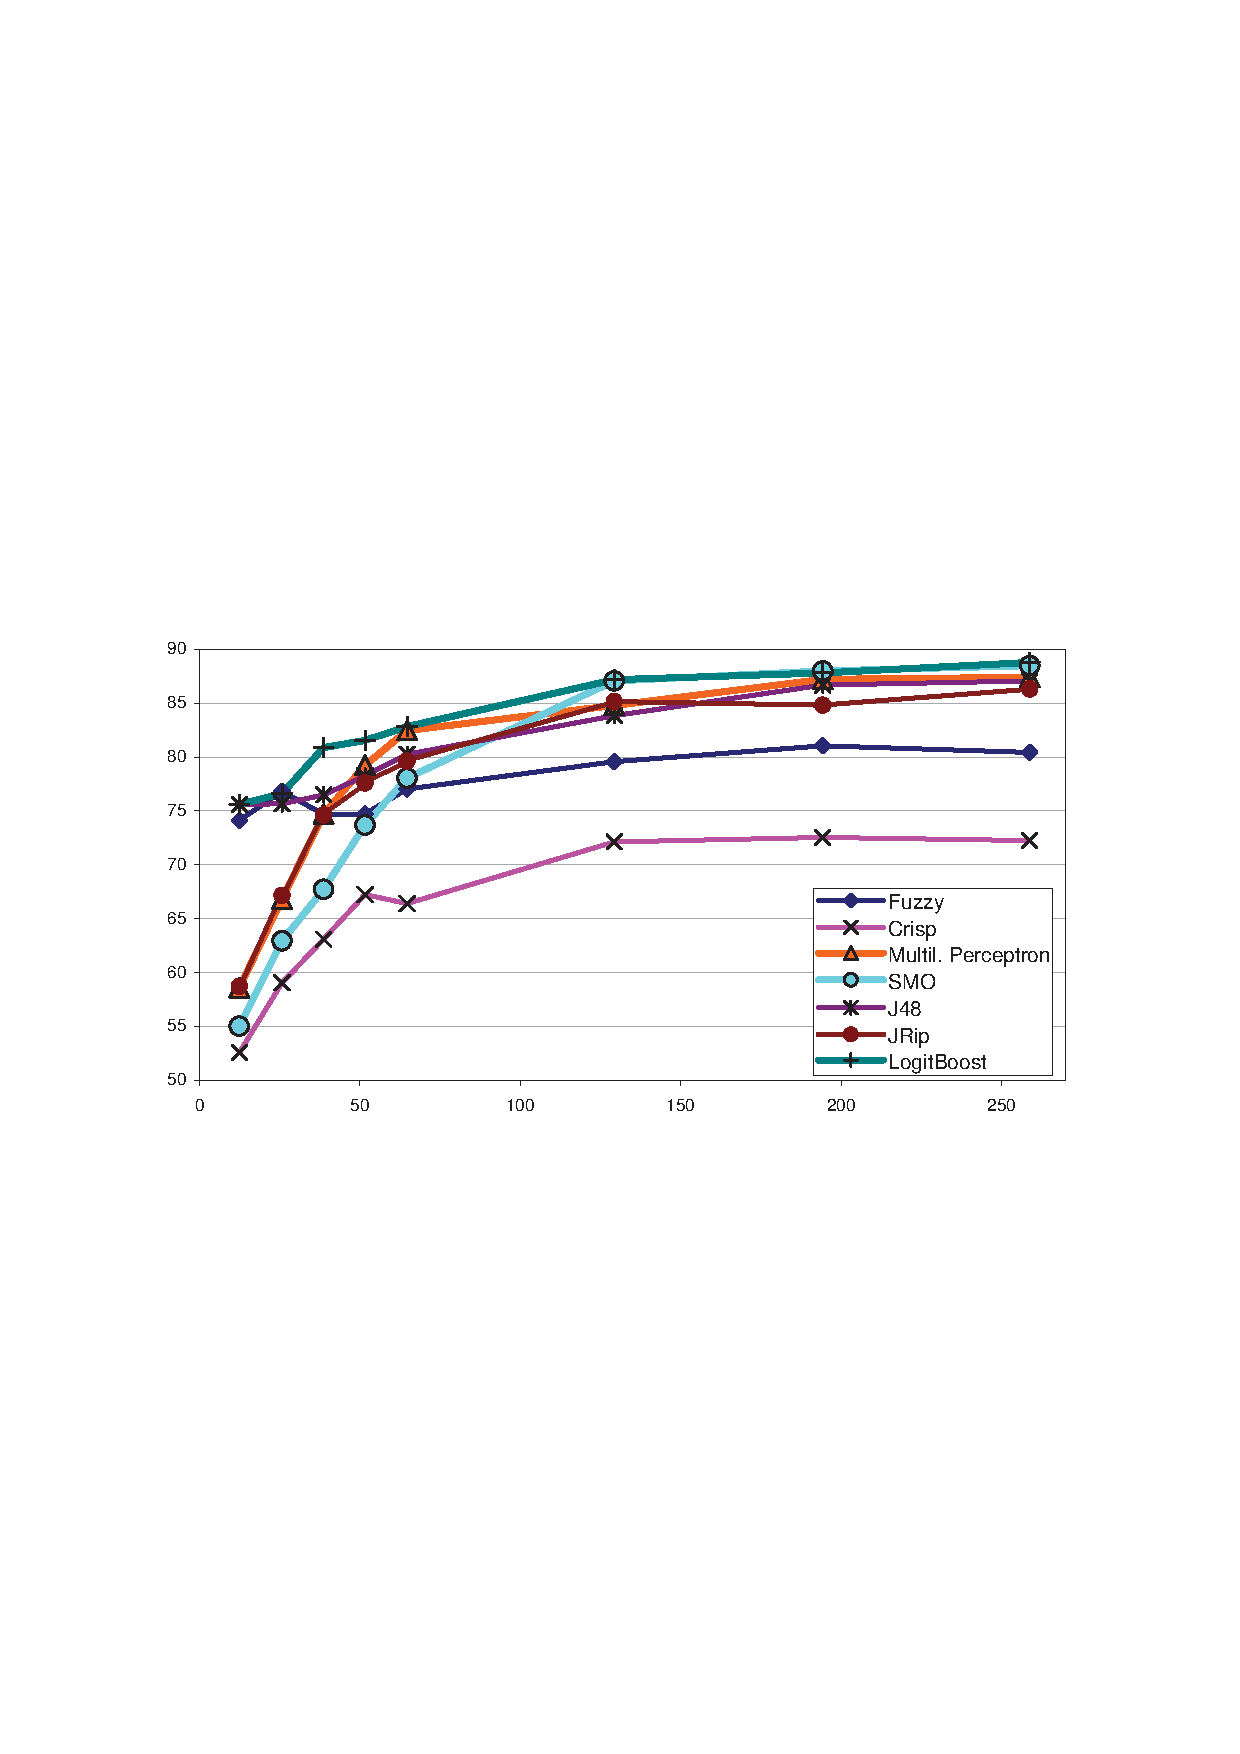
\includegraphics[width=0.8\hsize]{corect_growing_learninig_instances}}
\caption{x-axis: number of training instances, y-axis: percent of correctly classified instances, average values from 10 repetitions, `nursery' dataset.}
\label{img:corect_growing_learninig_instances}
\end{figure}


\subsection{UCI Time}


Figure~\ref{img:learning_speed} demonstrates time complexity of the classifiers in the same experiment as in Figure~\ref{img:corect_growing_learninig_instances}. Despite the fact that the Fuzzy ILP classifier was several times slower than the Crisp ILP classifier and even more than the others, it is still computable on current processors (e.g. P9600, 2.66 GHz, which we used) and the curve of time complexity did not grow rapidly during the experiment. Because ILP is a heuristic and iterative method, the time complexity can be quite directly managed by the setting of learning parameters.

\begin{figure}
\centerline{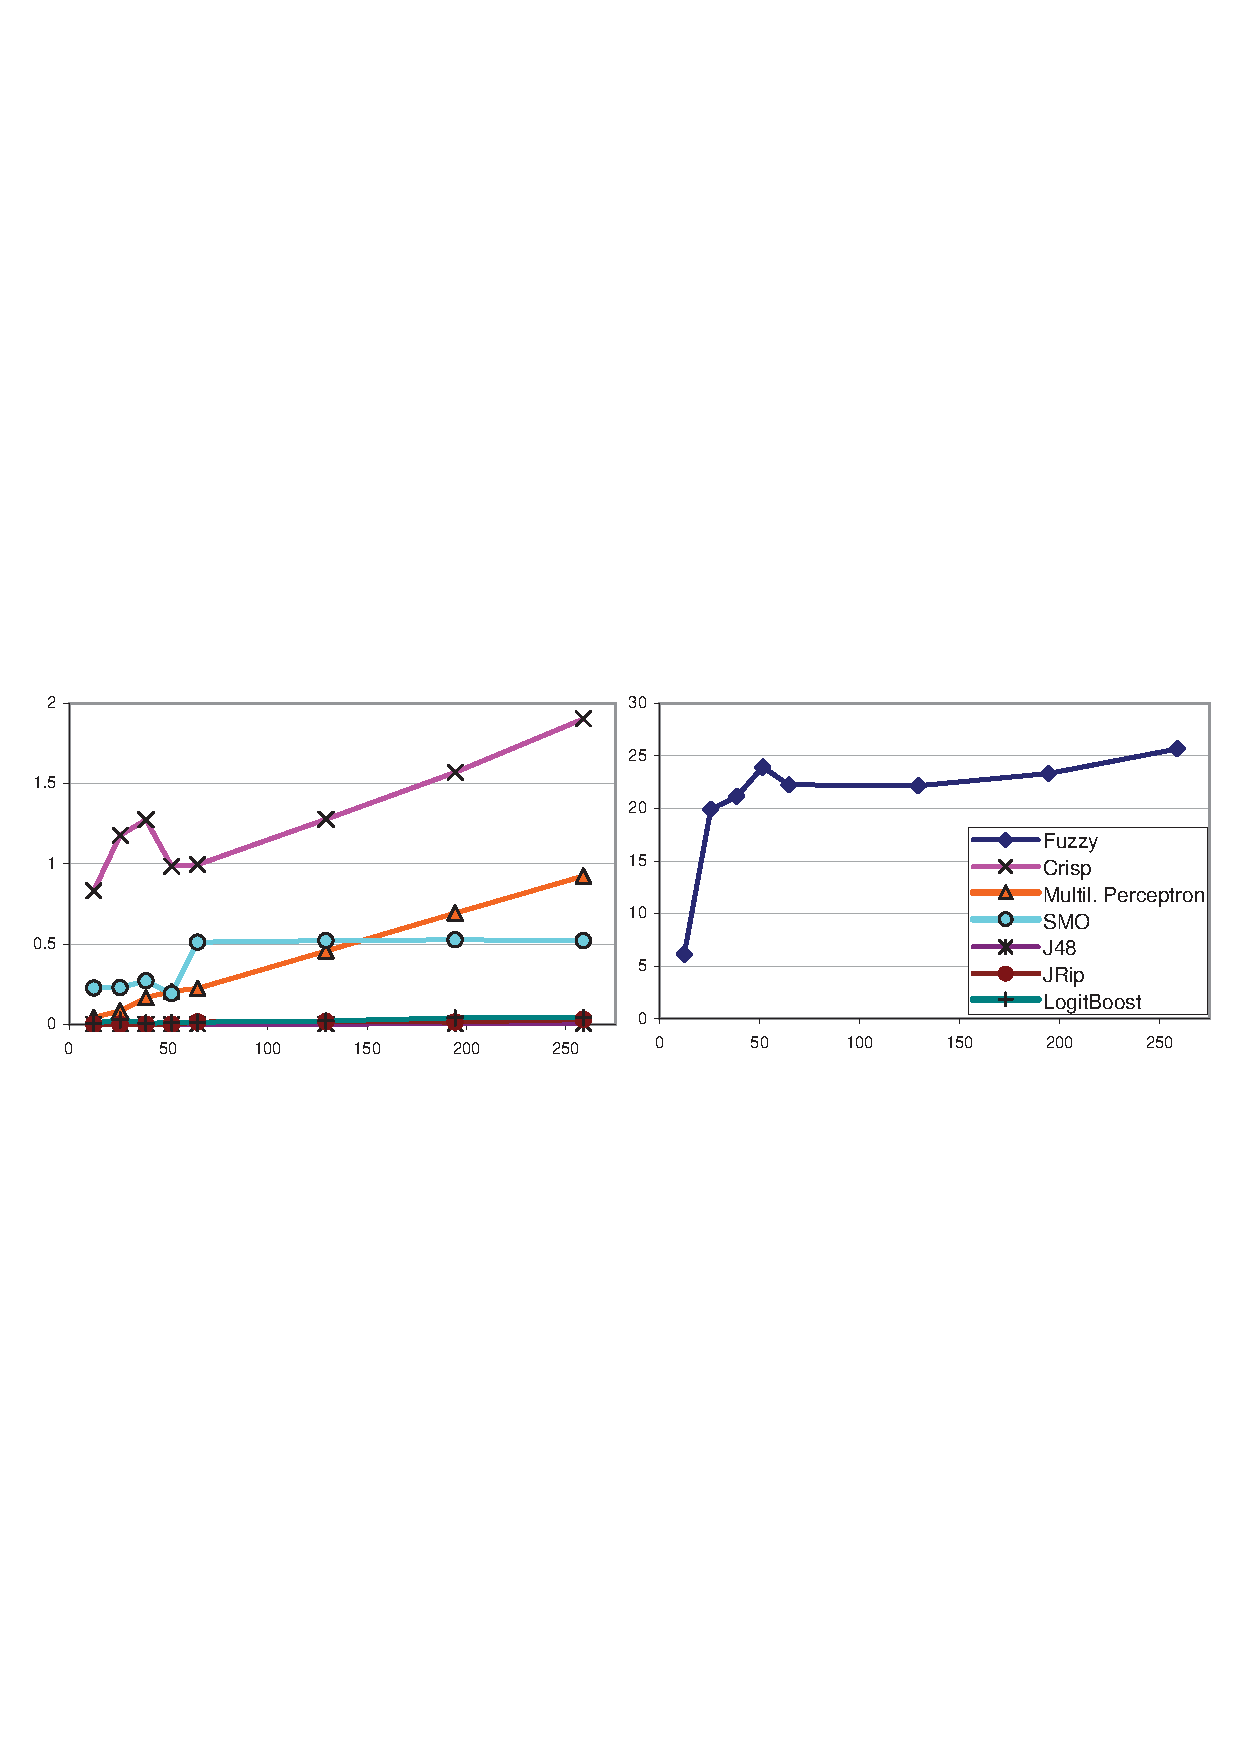
\includegraphics[width=\hsize]{learning_speed}}
\caption{x-axis: number of training instances, y-axis: training time in seconds, average values from 10 repetitions, `nursery' dataset.}
\label{img:learning_speed}
\end{figure}


